\documentclass{beamer}

\usetheme{CambridgeUS}

\usepackage{amsmath}
\usepackage{adjustbox}
\usepackage{amsmath}
\usepackage{amssymb}
\usepackage{relsize}
\usepackage{graphicx}
\usepackage{verbatim}
\usepackage{hyperref}
\usepackage{relsize}
\usepackage{amsthm}

\usepackage{pgffor}%
\usepackage{geometry}
\usepackage{pdflscape}

\usepackage[utf8]{inputenc}
\usepackage[english]{babel}


\newtheorem{proposition}[theorem]{Proposition}
\newtheorem{assumption}[theorem]{Assumption}

\title{Impacts of Taxes on Firm Location}
\author{Kevin D. Duncan}
\institute{Iowa State University}
\date{MVEA, Oct 22nd 2015}

\begin{document}

\begin{frame}
\title{Impacts of Taxes on Firm Entry Rates along State Borders}
\subtitle{A Border Discontinuity Approach}
\author{Kevin D. Duncan}
\institute{Iowa State University}
\date{Missouri Valley Economics Association \\ October 22nd, 2015}
\maketitle
\end{frame}

\begin{frame}
\section{Introduction \& Motivation}
\frametitle{Introduction}
Our paper studies the following two problems
\begin{itemize}
\item Do changes in tax and regulatory policy impact firm entry?
\item Do firms have preferences for government provided amenities?
\end{itemize}

How we accomplish this task
\begin{itemize}
\item We take differences in firm startup rates between matched county-pairs on either side of a state border.
\item This model relies on entrepreneuers picking firm entry locations between a close set of possible locations along state borders.
\item We employ the difference in top marginal tax rates as the relevant tax rates that many entrepreneurs pay.
\end{itemize}

\end{frame}


\begin{frame}
\section{Motivation}
\frametitle{Motivation}
Our motivation
\begin{itemize}
\item Older papers explored firm entry across all counties, but policy endogeneity between tax rates and economic activity upwards biases these estimates. Border discontinuity approaches solve this problem.
\item  Many papers do not include marginal tax rates, or only include a few tax types.
\item Theory indicates that marginal rates are what matter, and tax rates might be jointly changed in order to achieve policy goals. We see this empirically as there is very strong correlations among certain tax rates leading to plausible ommitted variable bias. Thus adding in a longer array of tax types might fix issues with ommitted variable bias.
\end{itemize}
\end{frame}

\begin{frame}
\section{Literature Review}
\frametitle{Literature Review}
\begin{itemize}
\item Early papers used conditional logit models to estimate firm entry across all counties. Often found positive relationship between taxes and firm entry rates. Carlton (1979, 1983), Schmenner (1975, 1982).
\item Modern papers have started to use border discontinuity effects to look at impacts of policies on firm entry rates. Chirinko and Wilson (2008), Rathelot and Sillard (2008), Duranton et al (2011), Rohlin, Rosenthal, and Ross (2014)
\item Across all papers there has been a variety of taxes used. 
\begin{itemize}
\item  Carlton (1983) used top marginal tax rates for corporate and income tax, but weighted them together, as well as property tax rates. 
\item Schmenner (1987) uses state and local property tax revenues per dollar of personal income. 
\item Helms (1985) used a budget constraint to estimate the impacts of rising tax revenue on explanatory variables.
\end{itemize}
\item all three approaches have modern equivalents, though theory shows that marginal tax rates are what matter!
\end{itemize}
\end{frame}

\begin{frame}
\section{Theory}
\frametitle{Theory Pt I}
\begin{itemize}
\item  Wages and capital costs are adjusted to local tax and location specific measures affecting firm level productivity. If markets are competitive firms will make zero economic profit in the long run, but demand or policy shocks leave short term profits.
\item If a regime changes its taxes, higher production costs and lower profits exist in that county. Thus that market will deter a relative amount of firms from entering as firms enter and bid up prices on the other side.
\item Firms make decisions based on information from the previous year, as governments might concurrently change policy along with market entry, and there are time costs associated with starting up a firm.
\end{itemize}
\end{frame}

\begin{frame}
\frametitle{Theory Pt II}
\begin{assumption}
Assume that a firms' profit can be expressed as a linear function, for a given location, state, and time pair denoted $(i,j,t)$,
\begin{equation}
\pi_{i,j,t} =  \gamma+\beta_{i}+\beta_{j}+X_{i,t-1}\beta_{1}+X_{j,t-1}\beta_{2}+\epsilon_{i,j,t}
\end{equation}
\begin{equation}
E[\epsilon_{ijt}] = 0
\end{equation}
$X_{i,t-1}$ is a $1 \times K_{1}$ row vector of location specific terms, and $X_{j,t=1}$ is a $1 \times K_{2}$ row vector of state specific terms, and $\beta_{i}, \beta_{j}$ are location and state specific fixed effects.
\end{assumption}
\end{frame}

\begin{frame}
\frametitle{Theory Pt III}
Now let us focus on a market that is defined by the interval $[-1,1]$, such that for $i \in [-1,0)$ a firm is in state $A$, and for $i \in [0,1]$, they are in state $B$. Therefore, if a firm has two choices, $y \in [-1,0)$ and $\hat y \in [0,1]$, then the firm chooses $y$ over $\hat y$ if
\begin{equation}\label{diff}
E[\pi_{y,A,t}-\pi_{\hat y,B,t}] > 0
\end{equation}

\begin{assumption}\label{cont}
$\beta_{i}$ and $X_{i,t-1}$ are continuous locally on $[-1,1]$, such that for any $\epsilon > 0$, where  $\max\{|\beta_{i}-\beta_{j}|,|(X_{y,t-1}-X_{\hat y,t-1})| \} < \frac{\epsilon}{2}$, then there exists a $\delta$ such that $|y - \hat y| < \delta$
\end{assumption}

Then we see that as $y,\hat y \to 0$ the choice becomes;
$$ E[\pi_{y,A,t}-\pi_{\hat y,B,t}] = (X_{A,t-1}-X_{B,t-1})\beta_{2} > 0$$
\end{frame}

\begin{frame}
\section{Data}
\frametitle{Data}
\begin{itemize}
\item Total number of firm start ups in every continental US county
\item Seven different state top marginal tax rates
\begin{itemize}
\item property, income, capital gains, sales, corporate, workers compensation, unemployment insurance
\end{itemize}
\item Log state expenditures per capita on education, highways, and welfare
\item Scaled county geographic amenities
\item Additional (state level) Controls: County level real fuel prices, pct with high school  education, population density, pct unionized, pct manufacturing
\end{itemize}
\end{frame}

\begin{frame}
\begin{figure}[h]\label{rb}
    \centering
    \textbf{Example of Border Matching}
    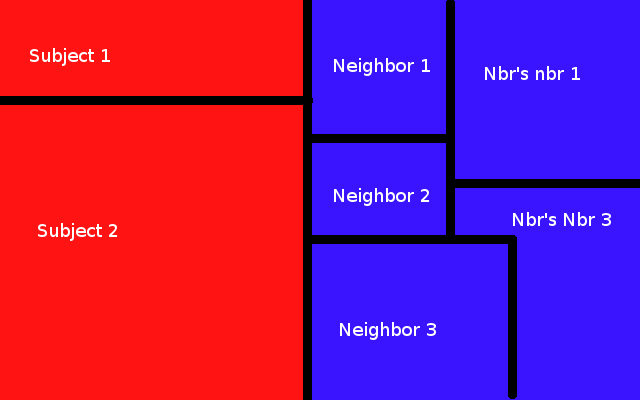
\includegraphics[scale = 0.35]{../../analysis/output/borders_temp.png}
    \caption{Red rectangles are subject counties, and blue are neighbor counties. In this example Subject 1 would be only matched to Neighbor 1, while "Subject 2" would be paired with Neighbor 1-3. Similarly, when we broaden the bandwidth, Subject 1 would be matched with Nbr's Nbr 1, whle Subject 2 would be paired with Nbr's Nbr 1 and 2}
\end{figure}
\end{frame}

\begin{frame}
\subsection{Regression Discontinuity Model}
\frametitle{Regression Discontinuity Model pt I}
\begin{itemize}
\item From our theory we show how the location effect drops out as we approach the border. we primarily estimate two models, first, a model without fixed effects,
\end{itemize}

\begin{equation} \label{pols}
\ddot ln(n_{i,g,t}) = \ddot x_{g,t-1}\beta_{2} + \ddot \epsilon_{i,g,t}
\end{equation}
 $$\ddot{ln(n_{i,g,t})} = ln(n_{sub,A,t})-ln(n_{nbr,B,t})$$
 $$\ddot x_{g,t-1} = x_{A,t-1}-x_{B,t-1}$$
 $$\ddot \epsilon_{i,g,t} = \epsilon_{sub,A,t}-\epsilon_{nbr,B,t}$$
\begin{itemize}
\item Secondly, we estimate a model that allows for an intercept for each state-pair.
\end{itemize}
\begin{equation}\label{fe}
\ddot \ln(n_{i,g,t}) = \beta_{A}-\beta_{B}+\ddot X_{g,t-1}\beta_{2} + \ddot \epsilon_{i,g,t}
\end{equation}


\end{frame}





\begin{frame}
\frametitle{RD Results}
% Table created by stargazer v.5.2 by Marek Hlavac, Harvard University. E-mail: hlavac at fas.harvard.edu
% Date and time: Tue, Oct 13, 2015 - 02:44:06 PM
\begin{table}[!htbp] \centering 
  \caption{Regression Discontinuity Models for  Total Firm Births} 
  \label{--rd} 
  {\tiny\renewcommand{\arraystretch}{.8}
\resizebox{!}{.35\paperheight}{%
\begin{tabular}{@{\extracolsep{5pt}}lcccc} 
\\[-1.8ex]\hline 
\hline \\[-1.8ex] 
 & \multicolumn{4}{c}{\textit{Dependent variable:}} \\ 
\cline{2-5} 
\\[-1.8ex] & \multicolumn{3}{c}{births ratio} & births\_ratio \\ 
 & OLS & OLS & OLS & FE \\ 
\\[-1.8ex] & (1) & (2) & (3) & (4)\\ 
\hline \\[-1.8ex] 
 Property Tax Difference & $-$0.206 & $-$0.371$^{**}$ & $-$0.297$^{**}$ & 0.027 \\ 
  & (0.151) & (0.147) & (0.150) & (0.122) \\ 
  Income Tax Difference & $-$0.093$^{***}$ & $-$0.085$^{***}$ & $-$0.075$^{***}$ & $-$0.009 \\ 
  & (0.027) & (0.026) & (0.026) & (0.035) \\ 
  Capital Gains Tax Difference & 0.016 & 0.008 & 0.020 & $-$0.002 \\ 
  & (0.023) & (0.023) & (0.024) & (0.012) \\ 
  Sales Tax Difference & $-$0.112$^{***}$ & $-$0.101$^{***}$ & $-$0.087$^{***}$ & 0.001 \\ 
  & (0.029) & (0.030) & (0.032) & (0.041) \\ 
  Corp Tax Difference & 0.023 & 0.018 & 0.011 & $-$0.012 \\ 
  & (0.020) & (0.018) & (0.019) & (0.026) \\ 
  Workers Comp Tax Difference & 0.001 & 0.090 & 0.051 & 0.044 \\ 
  & (0.111) & (0.108) & (0.105) & (0.070) \\ 
  Unemp. Tax Difference & 0.008 & 0.012 & $-$0.006 & $-$0.002 \\ 
  & (0.040) & (0.036) & (0.038) & (0.017) \\ 
  Educ Spending Per Cap Diff & $-$0.0002 & $-$0.0003 & $-$0.0002 & $-$0.0002 \\ 
  & (0.0003) & (0.0003) & (0.0003) & (0.0002) \\ 
  Highway Spending Per Cap Diff & 0.0004 & 0.0004 & 0.0003 & 0.0001 \\ 
  & (0.0004) & (0.0004) & (0.0004) & (0.0002) \\ 
  Welfare Spending Per Cap Diff & 0.001$^{**}$ & 0.001$^{**}$ & 0.0004$^{*}$ & $-$0.00005 \\ 
  & (0.0003) & (0.0003) & (0.0003) & (0.0001) \\ 
  Constant & $-$0.045 & $-$0.055 & $-$0.046 &  \\ 
  & (0.084) & (0.086) & (0.087) &  \\ 
 \hline \\[-1.8ex] 
controls & Yes & Yes & No & Yes \\ 
amenities & Yes & No & No & No \\ 
\hline \\[-1.8ex] 
\hline 
\hline \\[-1.8ex] 
\end{tabular}}}
\end{table} 
\end{frame}

\begin{frame}
\subsection{Sensitivity Tests}
\frametitle{Sensitivity Tests}
\begin{itemize}
\item Stability of coefficients across years.
\item Symmetry of coefficients across borders.
\item Stability of coefficients across NAICS sub-codes.
\item Extending the distance between matched pairs.
\item Working on estimating main model for each US region.
\end{itemize}
\end{frame}


\begin{frame}
\section{Analysis}
\frametitle{Some Comparisons: Weighted Tax Differentials}
\begin{figure}[h]\label{weightedtax}
    \centering
    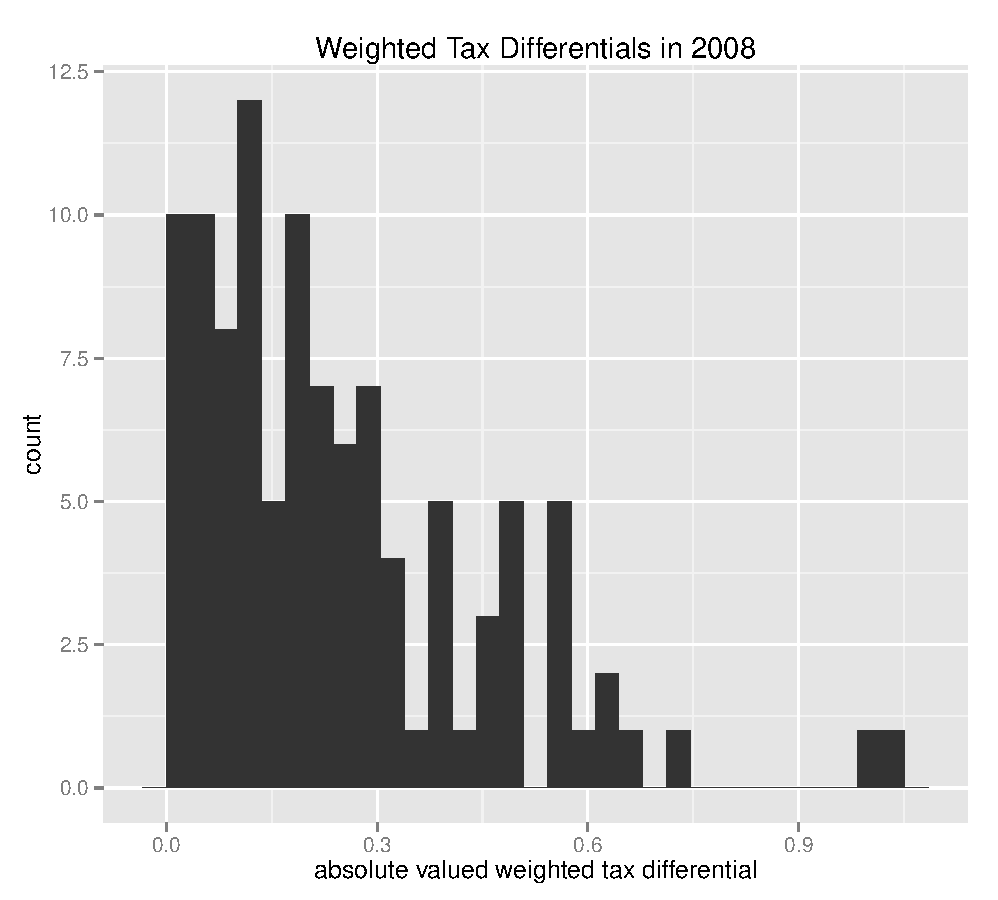
\includegraphics[scale = 0.5]{../../analysis/output/_--_weightedtax.pdf}
\end{figure}
\end{frame}

\begin{frame}
\frametitle{Some Comparisons Pt II}


% Table created by stargazer v.5.2 by Marek Hlavac, Harvard University. E-mail: hlavac at fas.harvard.edu
% Date and time: Mon, Feb 15, 2016 - 03:01:17 PM
\begin{table}[!htbp] \centering 
  \caption{Result Comparison for Total Firm Births} 
  \label{meantable} 
\tiny 
\begin{tabular}{@{\extracolsep{5pt}} ccccccc} 
\\[-1.8ex]\hline 
\hline \\[-1.8ex] 
mean firm entry & preffered side & abs weighted tax & preferred side & same? & sub state & nbr state \\ 
\hline \\[-1.8ex] 
$2.591$ & nbr & $0.010$ & sub & different & kansas & nebraska \\ 
$2.260$ & nbr & $0.016$ & nbr & same & maryland & west virginia \\ 
$2.194$ & sub & $0.294$ & sub & same & alabama & georgia \\ 
$2.126$ & sub & $0.205$ & nbr & different & minnesota & wisconsin \\ 
$1.808$ & sub & $0.097$ & nbr & different & ohio & pennsylvania \\ 
$1.743$ & sub & $0.555$ & sub & same & colorado & kansas \\ 
$1.568$ & nbr & $0.105$ & nbr & same & arizona & nevada \\ 
$1.513$ & nbr & $0.256$ & sub & different & idaho & utah \\ 
$1.477$ & sub & $0.119$ & sub & same & oklahoma & texas \\ 
$1.376$ & nbr & $0.015$ & nbr & same & kentucky & west virginia \\ 
\hline \\[-1.8ex] 
\end{tabular} 
\end{table} 


\end{frame}

\begin{frame}
\section{Conclusion}
\frametitle{Conclusion}
Going back to our original two research questions, we see that:
\begin{itemize}
\item Property, sales, and income taxes across most specifications besides for our interaction term regressions. 
\item Property tax rates have a relatively high elasticity, where a 1\% increase in relative property tax rates corresponds to a 0.49\% decrease in relative firm start up rates. A 1\% increase in relative sales and income tax rates correspond to a 0.08\% decrease in relative firm start up rates.
\item Government expenditures on infrastructure, welfare, and education does not seem to impact firm start up. rates.

\end{itemize}
\end{frame}

\begin{frame}
\begin{centering}
\huge{Thank you for your time!}
\end{centering}
\end{frame}
\end{document}